\documentclass{paper}

%\usepackage{times}
\usepackage{epsfig}
\usepackage{graphicx}
\usepackage{amsmath}
\usepackage{amssymb}
\usepackage{color}
\usepackage{subcaption}
\usepackage{caption}


% load package with ``framed'' and ``numbered'' option.
%\usepackage[framed,numbered,autolinebreaks,useliterate]{mcode}

% something NOT relevant to the usage of the package.
\setlength{\parindent}{0pt}
\setlength{\parskip}{18pt}






\usepackage[latin1]{inputenc} 
\usepackage[T1]{fontenc} 

\usepackage{listings} 
\lstset{% 
   language=Matlab, 
   basicstyle=\small\ttfamily, 
} 



\title{Report Computer Vision Project 2}



\author{Single Michael\\08-917-445}
% //////////////////////////////////////////////////


\begin{document}



\maketitle


\section{Binocular Stereo (Due on 28/10/2014)}



\subsection{Epipolar lines Estimation (50 points)}
For given two images - called left and right - both showing a certain object from different viewing positions (i.e. Multiview geometry) we were supposed to estimate the epipolar lines in both images. Epipolar lines are the intersections of epipolar plane with the image plane. Furthermore, when selecting a point from the left image, our program should be able to estimate the corresponding point in the right image. \\

Initially, a user has to select a certain point in the left image and then mark the corresponding position in the right image by clicking at the appropriate position. For each click a user performs we store the corresponding image coordinates at the position where the user performed its click action and also remember from which image this click came from. We store these image coordinates as two dimensional homogenous positions. Remember that two-dimensional homogenous coordinates that represents a point in space have three components, where the last is equal one and the first two correspond to the regular cartesian coordinates of the clicked image position. A user has to mark in both images eight positions using our GUI, alternating, first in the left, then in the right image the corresponding position. The collected homogenous coordinates resulting from the selection-process in the left image are both stored in a $3 \times 8$ matrix called \emph{left} (each column represents a homogenous point). Similarly, the collected selections in the right image are stored in a $3 \times 8$ matrix called \emph{right}. \\

Using these \emph{left} and \emph{right} positions we compute (estimate) the fundamental matrix $F$ by applying the \emph{normalized eight point algorithm} on them. This algorithm is called \emph{normalized} since all selected positions from the left image and those from the right image are centred towards their mean center which is supposed to denote the approximate image origin $(0,0)$ (each image has its own origin). \\ 

The normalization process for a given set of points works as the following: using the (x,y) from a set of points (in our case a matrix carrying homogenous coordinates), we compute the mean position by summing all positions and dividing by the number of used points (in this exercise this is equal to eight points). Then, we shift all the given point positions towards this center by subtracting each position by their mean position. \\

In order to increase the numerical stability of the eight-point algorithm, we are supposed to ensure, that the mean squared distance between the origin (i.e. the mean position of the point set) and each point is equal to 2 pixels. \\

Thus, we also have to rescale each point in the left and in the right position collection by a factor $s = \frac{\sqrt{2}}{\bar{d}}$ where $\bar{d}$ denotes the average distance of all point distances (of the points in a certain point set) to their average position (i.e. their origin). Since we are using homogenous coordinates, we can formulate this \emph{position normalization} as a homogenous transformation, capturing a translation towards the average position, and a rescaling such that the mean squared distance to the origin is equal to two pixels. Formally, such a transformation looks like the following:

\begin{align*}
T = \left(\begin{array}{ccc}
s & 0 & -c_1 s \\
0 & s & -c_2 s \\
0 & 0 & 1 \\
\end{array} \right)
\end{align*}


Where the scaling factor $s$ is the distance scaling (such that the mean squared distance of each position to the origin is equal two pixels) and $(-s c_1, -s c_2)$ is the translation to the origin. \\

For both point sets, \emph{left} and \emph{right}, we have to compute such a homogenous transformation matrix. Then we have to apply these transformations to their points. We denote the normalization transformation for the left point set as $T_{l}$ and for the right point set as $T_{r}$. \\

Next, let us consider the two points $\textbf{x} = (u,v,1)^{T}$ and $\textbf{x'} = (u',v',1)^{T}$ where $\textbf{x}$ is a normalized point from the left image (using $T_l$) and $\textbf{x'}$ a normalized point from the right image. \\

Given the following epipolar constraint 

\begin{align}
    \textbf{x'}^{T} F \textbf{x} = 0
\label{eq:epipolar_constraint}
\end{align}

Where $F$ denotes the (yet) unknown Fundamental matrix we are looking for. By solving the minmizing problem 
\begin{align}
    \min_{\bf{F}} \sum^{N}_{k=1} \left(\textbf{x'}_{k}^{T} \textbf{F} \textbf{x}_{k}\right)^2 s.t. ||\textbf{F}||^2 = 1
\label{eq:min_problem}
\end{align}
 We we can therefore retrieve $F$. \\
 In the following I describe some further steps in detail how to compute the fundamental matrix $F$ using above's insights. \\

We start by explicitly showing all components in the epipolar constraint from equation $\ref{eq:epipolar_constraint}$: 

\begin{align}
\left(\begin{array}{ccc}
u' & v' & 1
\end{array}
\right)
\left(\begin{array}{ccc}
f_{11} & f_{12} & f_{13} \\
f_{21} & f_{22} & f_{23} \\
f_{31} & f_{32} & f_{33} \\
\end{array} \right)
\left(\begin{array}{c}
u \\
v \\
1
\end{array}
\right)
= 0
\label{eq:fundamental_matrix_block_form}
\end{align}

which is the same as

\begin{align*}
\left(\begin{array}{ccccccccc}
u' u & u' v & u' & v' u & v' v & v' & u & v & 1
\end{array}
\right)
\cdot
\left(\begin{array}{c}
f_{11} \\
f_{12} \\
f_{13} \\
f_{21} \\
f_{22} \\
f_{23} \\
f_{31} \\
f_{32} \\
f_{33}
\end{array}
\right)
= 0
\end{align*}

Let us define 

\begin{equation}
Y = 
\left(\begin{array}{ccccccccc}
u' u & u' v & u' & v' u & v' v & v' & u & v & 1
\end{array}
\right)
\end{equation}



and 

\begin{equation}
    f = \left(\begin{array}{c}
f_{11} \\
f_{12} \\
f_{13} \\
f_{21} \\
f_{22} \\
f_{23} \\
f_{31} \\
f_{32} \\
f_{33}
\end{array}
\right)
\end{equation}

thus, we solving 
\begin{equation}
 Y \cdot f = 0
\end{equation}

will solve the equation $\ref{eq:min_problem}$. Such a system of equations can usually be solved by using a SVD docompositon of the system. We choose f as the left singular vector that corresponds to the smallest singular value of $Y$. Thus let us apply the singular value decomposition on $Y$:

\begin{equation}
    Y = U \Sigma V^{T}
\label{eq:svd_y}
\end{equation}

Where U,V are orthonormal (rotation) matrices (i.e. $U U^{T} = I = U^{T} U$ same for V), and $\Sigma$ is a diagonal matrix containing all singular values of $Y$ in an ascending order. This means, the highest singular values is the first diagonal element, the smalles singular value is the last diagonal element of $\Sigma$. \\

Since we are interested in the left singular vector that corresponds to the the smallest singular values in $\Sigma$ we have to take the last column of $U$. Therefore we assign f by the last column of U, i.e. 

\begin{equation}
    f = \left(\begin{array}{c}
U_{19} \\
U_{29} \\
U_{39} \\
U_{49} \\
U_{59} \\
U_{69} \\
U_{79} \\
U_{89} \\
U_{99}
\end{array}
\right)
\end{equation}
 
Going back to the definition from equation $\ref{eq:fundamental_matrix_block_form}$ of the fundamental matrix $F$ we get

\begin{align}
\left(\begin{array}{ccc}
U_{19} & U_{29} & U_{39} \\
U_{49} & U_{59} & U_{69} \\
U_{79} & U_{89} & U_{19} \\
\end{array} \right)
\end{align}


Next we have to enforce the rank-2 constraint by setting the smallest singular value of F's SVD to zero. Formally, this corresponds to decompose F into its SVD components, set the last component of its matrix $\Sigma$ to zero and compute 

\begin{align}
    F_{rank=2} = U \Sigma' V^{T}
\end{align}

where $\Sigma$ denotes the modified $3 \times 3$ singular value diagonal matrix $\Sigma$ with the last singular value set to zero. \\

the last remaining step is to transform the fundamental matrix $F_{rank=2}$ back to original units. This can be achieved by multiplying the point-set normalization matrices $T_l$ and $T_r$ to $F_{rank=2}$:

\begin{equation}
    F = T_{r}^{T} F_{rank=2} T_{l} 
\label{eq:fundamental_matrix_rank2_final}
\end{equation}

This final transformation undoes all previous unit transformations (resulted from transforming into left image, right image positions). The matrix $F$ from equation $\ref{eq:fundamental_matrix_rank2_final}$ denotes the Fundamental matrix fulfilling the rank two constraint used in order to estimate the epiplar geometry. \\

Next, we use $F$ and apply the following epipolar constraints to it:

\begin{align*}
F e = 0 \\
F^{T} e' = 0 
\end{align*}

Where $e$ is the epipole in the left image and $e'$ denotes the epipole in the right image. We can solve for $e$ and $e'$ by computing the kernel of the matrix $F$ and $F^{T}$ respectively. The cross product between the left epipole and any point in the left image gives us the the coefficients of a general line in a two dimensional space. This will us allow us to fit a line through the left image. \\

Mathematically, this corresponds to:

\begin{equation}
    (a,b,c) = e \times p_{left}
\end{equation}

and then we have to evaluate the line general line quation 

\begin{equation}
    ax + by + c = 0
\end{equation}

We solve this equation for $y$ using $x = [0,lengt(Image_{left})]$. \\

The corresponding epipole line on the right image can be obtained by applying the fundamental matrix to the point selected in the left image. This gives us a vector with three components. We again use these three components as line coefficients for a line though space. \\

In the following I demonstrate some sample results produced by my Matlab code:
\begin{itemize}
    \item The figures figure $\ref{fig:cow_userselection}$ (Cow) and figure $\ref{fig:zyt_userselection}$ (Zytglogge) visualize the feature points selected by a user. Each feature point selected on the left image should correspond to one point in the right image.
    \item The figure $\ref{fig:cow_userselection}$ shows the estimated epipolar line in the Cow image using the user specified image shown earlier and a new user selection in the left image (indicated as a cyan dot on the left red epipolar line). The blue line corresponds to the epipolar line on the right image. Similar plots of the epipolar line using the Zytglogge data-set are shown in the figures figure $\ref{fig:zyt_epipolarline_1}$, $\ref{fig:zyt_epipolarline_2}$ and $\ref{fig:zyt_epipolarline_3}$.
    \item Last we visualize the numerical plots of the epipoles of both our data-sets. Figure $\ref{fig:cow_epipole}$ shows the epipoles of the Cow data-set and figure $\ref{fig:zyt_epipole}$ shows the epipoles of the Zytglogge data-set.
\end{itemize}


% showing user selection
\begin{figure}[H]
\centering
\begin{subfigure}{0.49\textwidth}
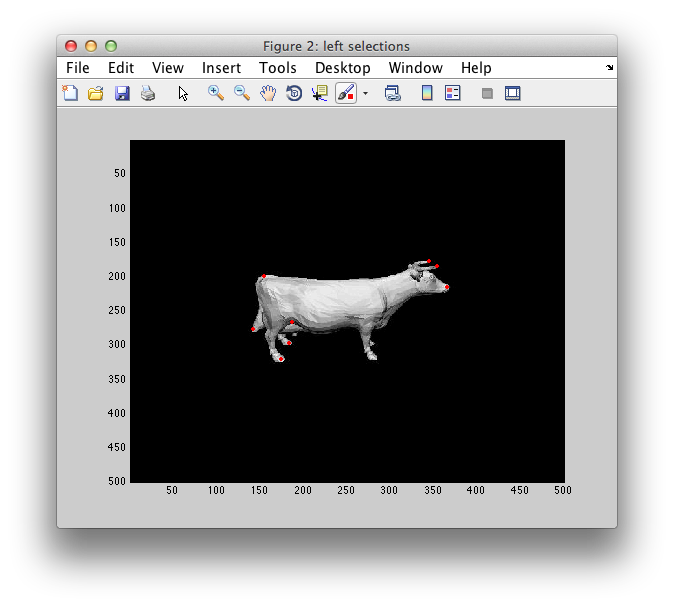
\includegraphics[width=\textwidth]{figures/cow_left_selected_points}
\end{subfigure}
\begin{subfigure}{0.49\textwidth}
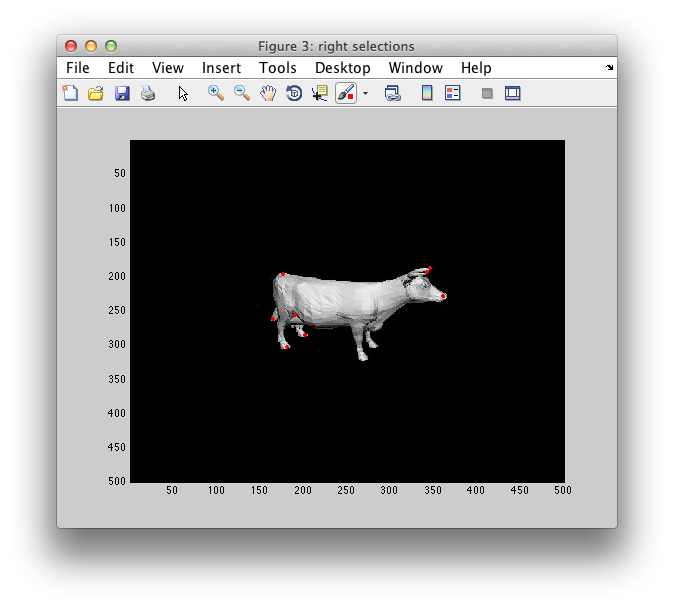
\includegraphics[width=\textwidth]{figures/cow_right_selected_points}
\end{subfigure}
\caption{Showing the eight user specified points in both cow images, the left image (on the left) and the right image (on the right.}
\label{fig:cow_userselection}
\end{figure}


\begin{figure}[H]
\centering
\begin{subfigure}{0.49\textwidth}
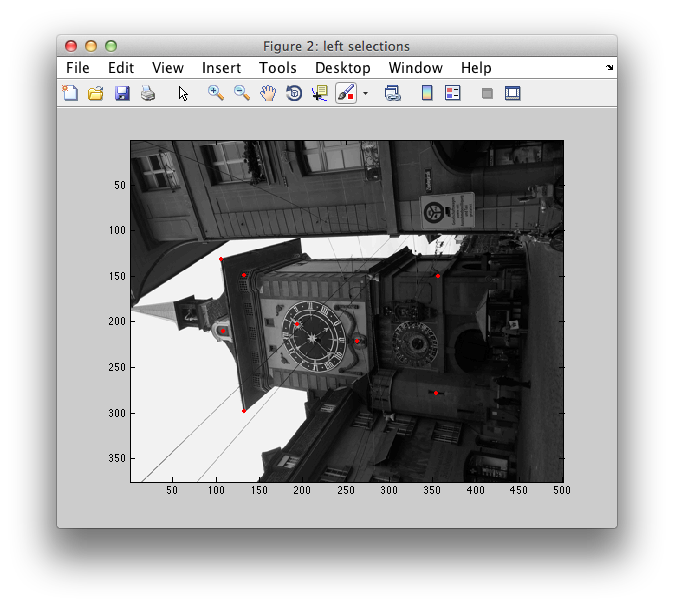
\includegraphics[width=\textwidth]{figures/zytglogge_left_selected_points}
\end{subfigure}
\begin{subfigure}{0.49\textwidth}
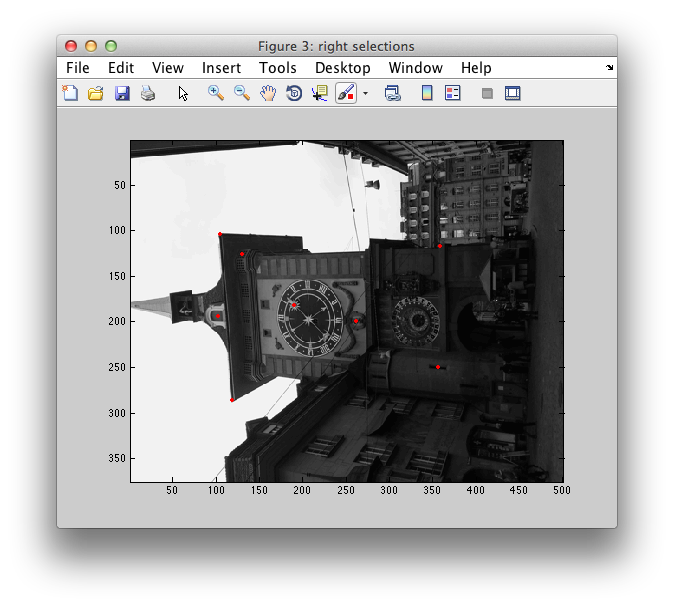
\includegraphics[width=\textwidth]{figures/zytglogge_right_selected_points}
\end{subfigure}
\caption{Showing the eight user specified points in both Zytglogge images, the left image (on the left) and the right image (on the right.}
\label{fig:zyt_userselection}
\end{figure}

% showing epipolar lines
\begin{figure}[H]
\centering
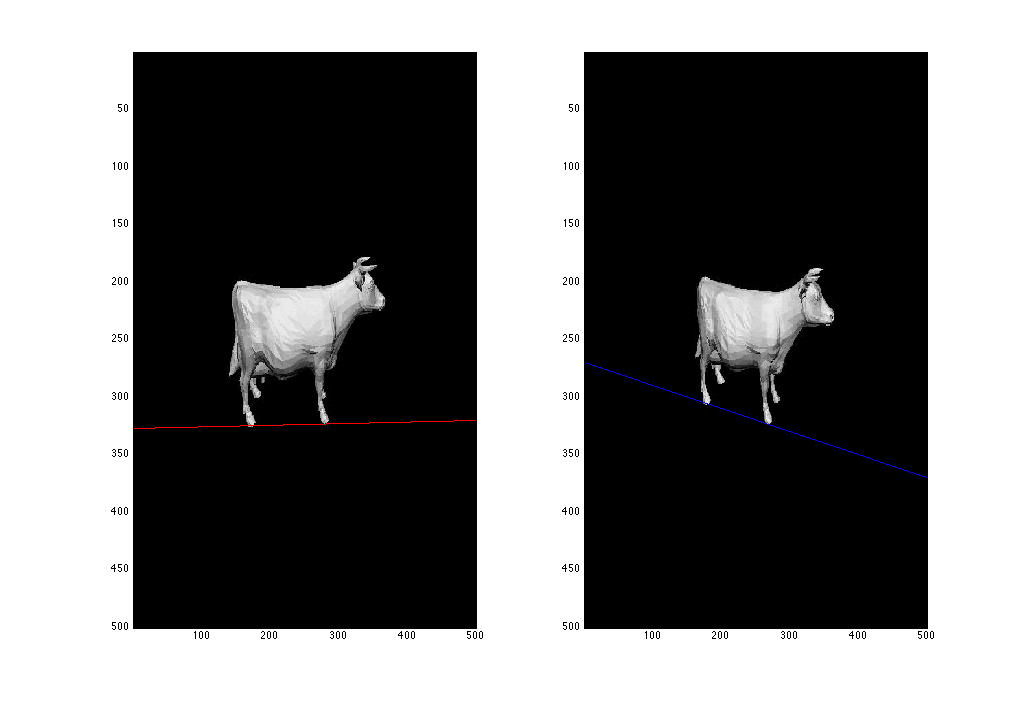
\includegraphics[width=\textwidth]{figures/epipolar_lines_cow}
\caption{Visualization of the estimated Epipolar Lines in both Cow images (left,red and right,blue) using a certain user selection which is indicated by a cyan colored little dot (you probably have to zoom-into the left image in order to see this dot) the left image.}
\label{fig:cow_epipolarline}
\end{figure}

\begin{figure}[H]
\centering
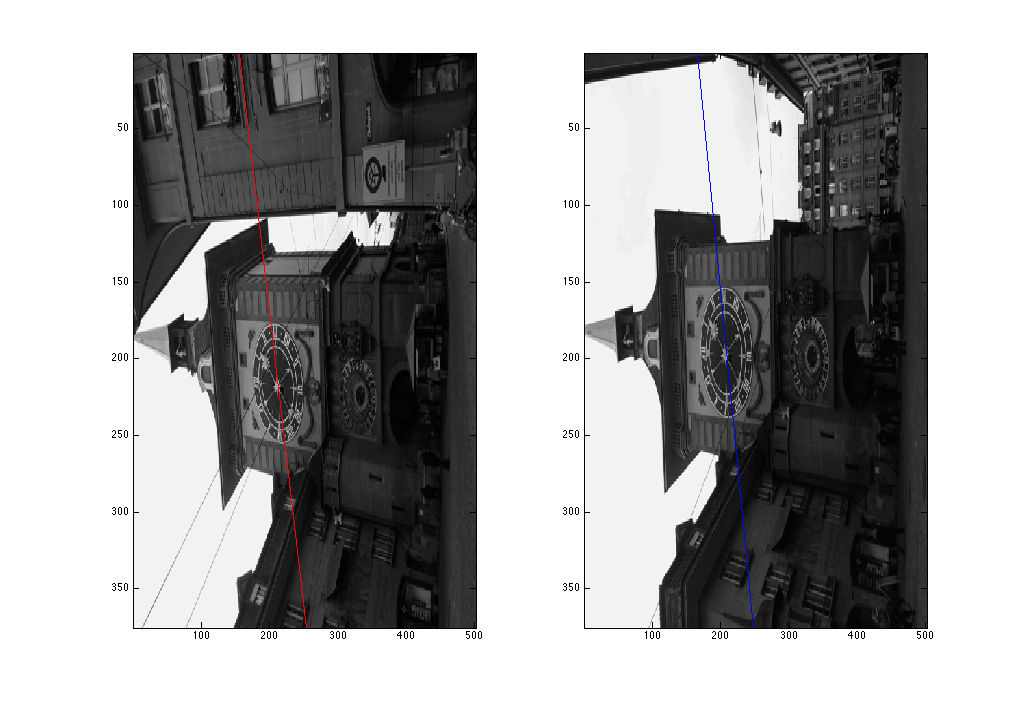
\includegraphics[width=\textwidth]{figures/epi_zyt_1}
\caption{Visualization of the estimated Epipolar Lines in both Zytglogge images (left,red and right,blue) using a certain user selection which is indicated by a cyan colored little dot (you probably have to zoom-into the left image in order to see this dot) the left image.}
\label{fig:zyt_epipolarline_1}
\end{figure}

\begin{figure}[H]
\centering
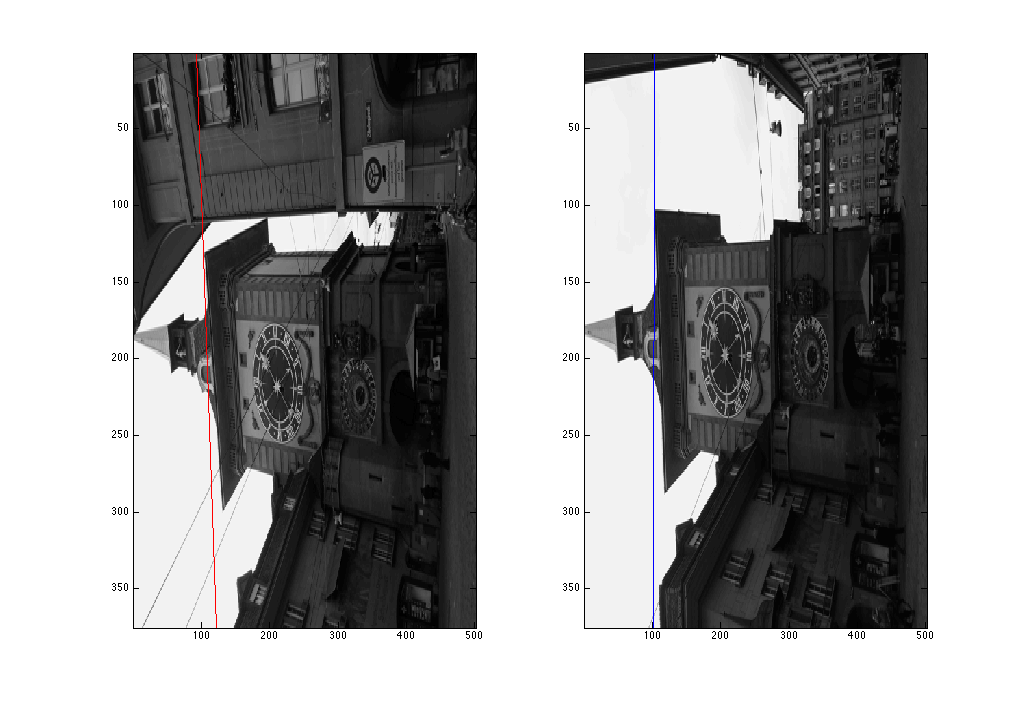
\includegraphics[width=\textwidth]{figures/epi_zyt_2}
\caption{Visualization of the estimated Epipolar Lines in both Zytglogge images (left,red and right,blue) using a certain user selection which is indicated by a cyan colored little dot (you probably have to zoom-into the left image in order to see this dot) the left image.}
\label{fig:zyt_epipolarline_2}
\end{figure}

\begin{figure}[H]
\centering
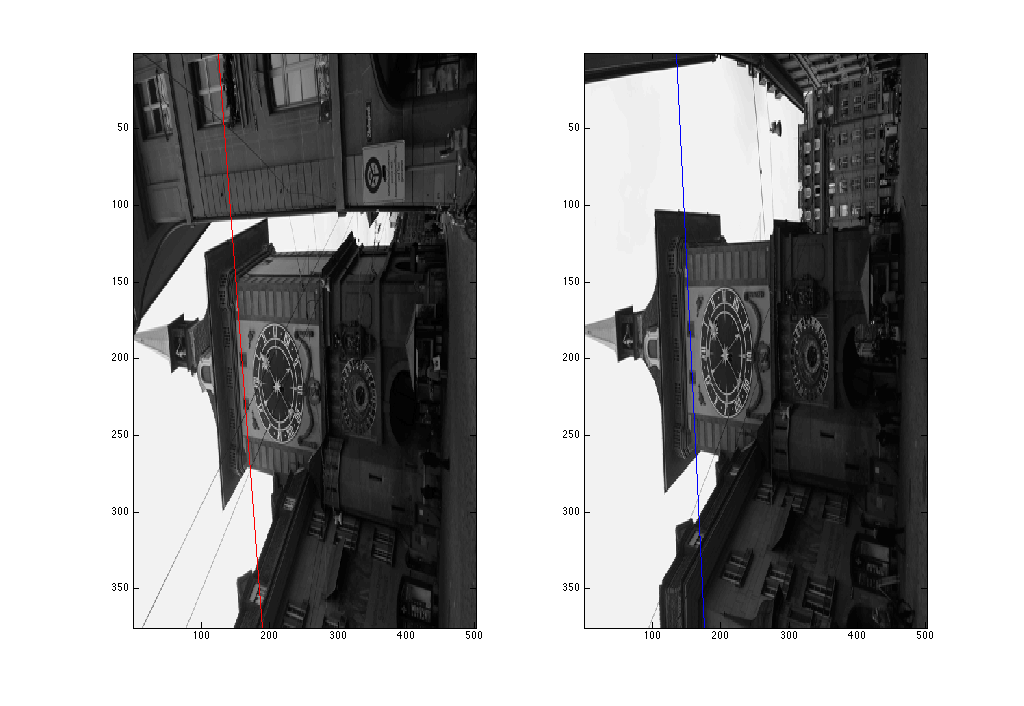
\includegraphics[width=\textwidth]{figures/epi_zyt_3}
\caption{Visualization of the estimated Epipolar Lines in both Zytglogge images (left,red and right,blue) using a certain user selection which is indicated by a cyan colored little dot (you probably have to zoom-into the left image in order to see this dot) the left image.}
\label{fig:zyt_epipolarline_3}
\end{figure}

% showing epipoles.
\begin{figure}[H]
\centering
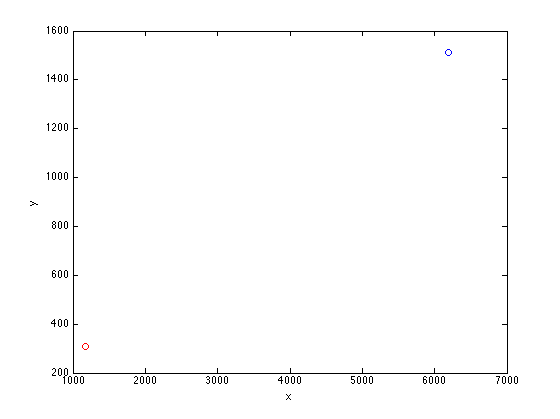
\includegraphics[width=\textwidth]{figures/epipole_cow}
\caption{Visualization of the coordinates of the epipoles of the Cow data-set. The red circle corresponds to the epipole in the left image, whereas the blue circle corresponds to the epipole in the right image.}
\label{fig:cow_epipole}
\end{figure}

\begin{figure}[H]
\centering
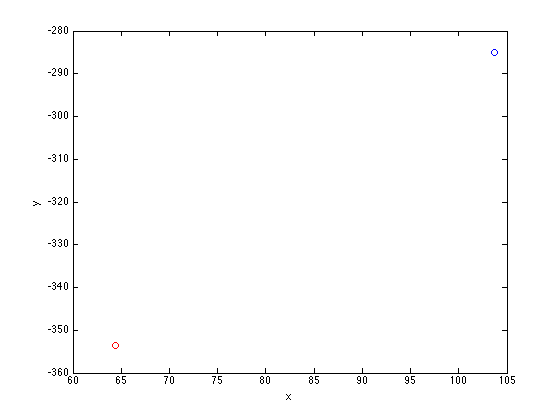
\includegraphics[width=\textwidth]{figures/epipole_zyt}
\caption{Visualization of the coordinates of the epipoles of the Zytglogge data-set. The red circle corresponds to the epipole in the left image, whereas the blue circle corresponds to the epipole in the right image.}
\label{fig:zyt_epipole}
\end{figure}



\subsection{Model reconstruction (50 points)}

From given (large) set of matching points of both cow-images, left and right, we want to reconstruct its corresponding 3d geometry by relying on the eight-point algorithm. Our goal is to estimate the depth of the given matching points. \\

In this task we are only provided by the intrinsic parameter $K$ which is describing the camera calibration. \\

We first estimate the fundamental matrix $F$, using all matching points from the provided data-set. Note that there are more than eight given points that we pass to our eight-point algorithm. \\

This gives us the following matrix for F:
\begin{align}
F = 
\left(\begin{array}{rrr}
   -0.0000  & -0.0000 &   0.0075 \\
   -0.0000  &  0.0000 &   0.0183 \\
    0.0001  & -0.0137 &  -1.9810 \\
\end{array} \right)
\end{align}

For solving this task we were provided by the camera calibration matrix $K$.  
Using the estimated Fundamental matrix $F$ we can compute the essential matrix $E$.

\begin{equation}
    F = K'^{-T} E K^{-1}
\label{eq:ektfk}
\end{equation}

In general, the essential matrix gives us the relative rotation and translation between the cameras of their extrinsic parameter. An illustration of this definition is shown in figure $\ref{fig:epipolar_constraints}$. \\

The provided matching points from both images were taken by the same camera. Thus, for our case $K$ is equal to $K'$. Thus, we simply can solve for $E$ in equation $\ref{eq:ektfk}$ which is thus equal to

\begin{align}
    E = K^{T} F K
\end{align}

When solving for the essential matrix in this task we get:

\begin{align}
E = 
\left(\begin{array}{rrr}
   -0.0005  & -0.1340 &  -0.2203 \\
   -0.0025  &  0.0188 &  -1.5708 \\
    0.0013  &  1.4839 &   0.0002 \\
\end{array} \right)
\end{align}

In the following let $x$ denote a point from the left image and $x'$ a point from the right image. From the class we know that the essential matrix is formed by a translation $[t]_x$ (that is expressed as a skew symmetric matrix and a rotation matrix $R$. 

\begin{align}
    E = [t]_x R 
\end{align}

\begin{figure}[h]
    \centering
    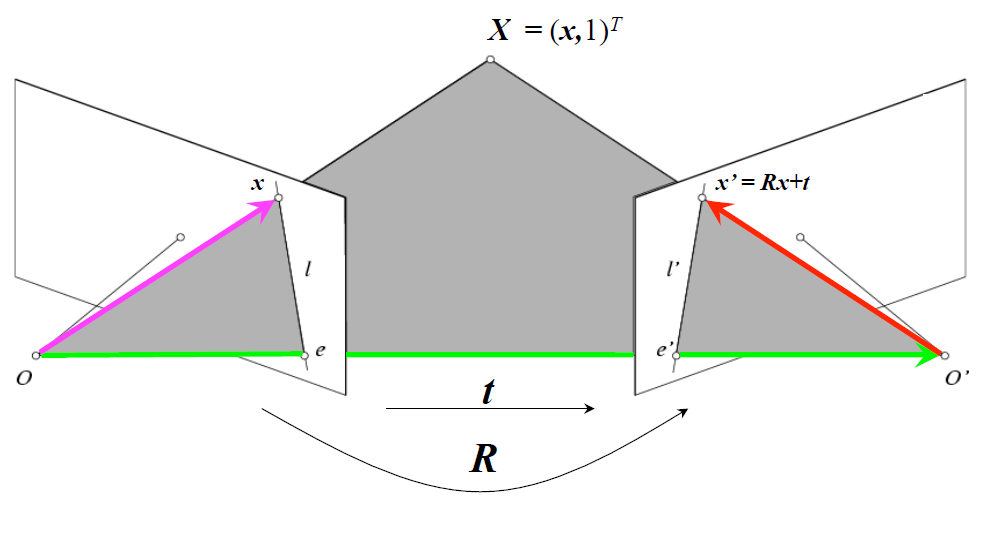
\includegraphics[width=\textwidth]{figures/epipol_const_cal_case}
    \caption{Illustration of the epipolar constraints for the calibrated case: The vectors $Rx$, $t$ and $x'$ are coplanar.}
    \label{fig:epipolar_constraints}
\end{figure}

Figure $\ref{fig:epipolar_constraints}$ again shows the epipolar constraint for the calibrated case and illustrated the relationship of the matrices $R$ and the translation vector $t$. 

\begin{align}
    x' \cdot \left( t \times R x \right) \rightarrow x' E x = 0
\end{align}

Thus, under ideal conditions, we can conclude, that the essential matrix $E$ is singular. Hence, we are going to compute the singular value decomposition (SVD) of the essential matrix:

\begin{align}
    E = U \Sigma V^{T}
\end{align}

In summary, we found that for the essential matrix (under ideal conditions) the following identities hold true:

\begin{equation}
    E = [t]_x R = U \Sigma V^{T}
\end{equation}

Under ideal conditions, the singular values stored in the $3 \times 3$ diagonal matrix $\Sigma$ are the same. However, in practise, the singular values differ due to various reasons such as numerical issues, not perfect calibrations and many more. Nevertheless, according to the rank-2 constraint on $F$, the last component singular value is equal to zero. \\

The diagonal entries of $\mathbf{\Sigma}$ are the singular values of $\mathbf{E}$ which, according to the internal constraints of the essential matrix, must consist of two identical and one zero value. Therefore we define 

\begin{align}
    R_{90} = 
    \left(\begin{array}{rrr}
       0  & -1 &  0 \\
       1  &  0 &  0 \\
       0  & 0 &  1 \\
\end{array} \right)
\end{align}

with 

\begin{align}
    R_{90}^{-1} = R_{90}^{T}
\end{align}




and make the following ansatz:

\begin{align}
    [t]_x = V R_{90} \Sigma V^{T} \\
    R = U R_{90}^{-1} V^{T}
\label{eq:ansatz}
\end{align}

Instead of using the provided definition of $[t]_x$ we can alter it to

\begin{align}
    [t]_x  = 
    \left(\begin{array}{r}
       U_{13} \\
       U_{23} \\  
       U_{33} \\
\end{array} \right)
\end{align}

Where we use the last column of us (which is paired with the smallest singular value, when multiplying the decomposition out) $U$ is the one component of the essential matrix' SVD. Thus, in short t corresponds to the last column of U up to a certain scaling. \\

Using the ansatz from equation $\ref{eq:ansatz}$ we just get one particular candidate solution. However there are more. Actually there exist four possible rotation transformation matrices and two possible translation matrices, i.e.

\begin{align}
    R = \pm U R_{90}^{\pm 1} V^{T} \\
    t = \pm 
        \left(\begin{array}{r}
       U_{13} \\
       U_{23} \\  
       U_{33} \\
\end{array} \right)
\end{align}

The cartesian product between $R$ and $t$ gives us the total number of candidate transformation solutions we have to examine. This is equal to eight candidate solutions. \\

It is possible to reduce the solution space we have to take into account to. We only take rotation transformation matrices that have a determinate equal to one (i.e. they exhibit a positive rotation orientation). Remember that the determinant of a matrix describing a rotation is always either equal one or equal to minus one. Considering the possible sign and transpose combinations we see that there will always two rotation matrices having a determinant equal to one and the other two equal to minus one. \\

For the remaining solution candidates, we reconstruct their depth $z$ - following the procedure as described below and take the rotation-translation combination exhibiting the most points lying in front of the camera (i.e. having a positive z-value/depth value). \\

Last we want to reconstruct 3d points $(x,y,z)$ from corresponding image points. More precisely, we want to compute the 3d points given corresponding normalized image coordinates 

\begin{align}
    \textbf{p}^{l} = (p^{l}_{x}, p^{l}_{y})
\end{align}

from the left image and image coordinates from the right image
\begin{align}
    \textbf{p}^{r} = (p^{r}_{x}, p^{r}_{y})
\end{align}

Assuming that the essential matrix $E$ is known and the corresponding rotation $R$ and translation $t$ transformations have been determined, we can apply the algorithm from Longuet-Higgins's Paper. \\

In the following let $r_k$ denote the k-th row of the rotation transformation $R$.



Combining the above relations between 3D coordinates in the two coordinate systems and the mapping between 3D and 2D points described earlier gives

\begin{align}
    p^{r}_{x} 
    &= \frac{x}{z} \\
    &= \frac{\mathbf{r}_{1} \cdot (\textbf{p}^{l} - \mathbf{t}/z)}{\mathbf{r}_{3} \cdot (\textbf{p}^{l} - \mathbf{t}/z)}  
\end{align}


Reformulating equation $\ref{eq:3d_reconstr_eq}$ we can solve for the height component $z$ from the 3d points as the following:

\begin{equation}
    z =  \frac{ (\mathbf{r}_{1} - p^{r}_{x} \, \mathbf{r}_{3}) \cdot \mathbf{t} }{ (\mathbf{r}_{1} - p^{r}_{x} \, \mathbf{r}_{3}) \cdot \textbf{p}^{l} }
\end{equation}


\begin{align}
\begin{pmatrix} x \\ y \end{pmatrix} = z \cdot \textbf{p}^{l}
\label{eq:find_x_y_3d_points}
\end{align}


In practise we also have to take the focal length $f$ of the camera in order to perform the computations stated in equation $\ref{eq:find_x_y_3d_points}$. Thus in practise we compute the following:

\begin{enumerate}
    \item $\forall \textbf{p}^{l}, \textbf{p}^{r}: z = \frac{ (\mathbf{r}_{1} - p^{r}_{x} \, \mathbf{r}_{3}) \cdot \mathbf{t} }{ (\mathbf{r}_{1} - p^{r}_{x} \, \mathbf{r}_{3}) \cdot \textbf{p}^{l} }$
    \item $\forall \textbf{p}^{l}: (x,y) = \frac{z \cdot \textbf{p}^{l}}{f}$
\end{enumerate}

The resulting, reconstructed 3d points $(x,y,z)$ are then plotted using Matlab's scatter3 function that allows us to illustrate a reconstructed image as a point cloud (without the need of performing a mesh triangulation). \\

In the following I am going to show some reconstruction images using the method described in this report, when running my code. I also compare my result to those one would get when knowing the exact rotation and translation matrices. These matrices are given as extrinsic parameters in order to compare the results. \\

The figures figure $\ref{fig:cow_rec_us_1}$, figure $\ref{fig:cow_rec_us_2}$, figure $\ref{fig:cow_rec_us_3}$ and figure $\ref{fig:cow_rec_us_4}$ show the reconstructed 3d points using our estimated rotation translation matrix $R$ and estimated translation vector $t$. Figure $\ref{fig:cow_rec_rltl}$ shows the reconstructed 3d points using the given $R_l$ and $t_l$ data. Last, figure $\ref{fig:cow_rec_rrtr}$ shows the reconstructed 3d points we get when using the given $R_r$ and $t_r$ data. \\

We observe that when we are using $R_r$ and $t_r$ for the 3d point reconstruction we obtain a cow that has almost no depth, i.e. this model is pretty flat. In contrary, when we are using the $R_l$ and $t_l$ data for the reconstruction process, we get an image which has appropriate depth values. This mean using $R_l$ and $t_l$ for the 3d reconstruction gives us a good looking 3d model having viable, visually convincing depth values. Applying our estimated $R$ and $t$ data gives us a reconstruction that produces depth values that are somewhere in between the both previous results. Using our data, the reconstructed model does not look that flat as when we were using $R_r$ and $t_r$. However, our reconstructed 3d points also do not exhibit depth details as when we were using $R_l$ and $t_l$. In my honest opinion, our reconstruction looks closer to the flat results when using $R_r$ and $t_r$. \\

Potential causes for this not that well looking results, when using our data:
\begin{itemize}
    \item Idea 1: The singular were differing too much from each other. The estimation approach we are using in order to reconstruct R assumes, that the singular values of the svd of the fundamental matrix are the same. Thus, when having a different $\Sigma$ sigma matrix as it was supposed to be there (having the same singular value twice (last singular values is zero - rank 2 constraint)). This also will affect the $U$ and $V$ matrices of the SVD of $F$, which we are using in order to compute $R$ and $V$. One possible solution to this problem would be some kind of rescaling or we could overwrite the 2nd singular value by the largest one. I have not tried this out - this is just an idea.
    \item there is a bug present: Even this is possible I do not think this is the result for this kind of difference. At least I have verified that I have computed matrices that describe a rotation (all their determinant is equal to $\pm 1$).
    \item Maybe the eight point algorithm is not sufficient enough in order to produce viable results. Even we use normalized points, we maybe should rely on a non-linear approach.
    \item Maybe there is noise present. However, I exclude this possibility, since then, in my opinion, none of our reconstructions should be able to produce nice depths.
    \item Maybe there is some kind of normalization issue still present, regarding the image normalization.
\end{itemize}

In general, the eight-point algorithm is very sensitive to the presence of noise. This means if there was noise to the correspondence, the results would look very different from those we obtained. Furthermore, when using de-normalized matching-points, the eight point algorithm would also perform rather bad due to numerical instabilities.

% showing reconstructions using our estimated matrices
\begin{figure}[H]
\centering
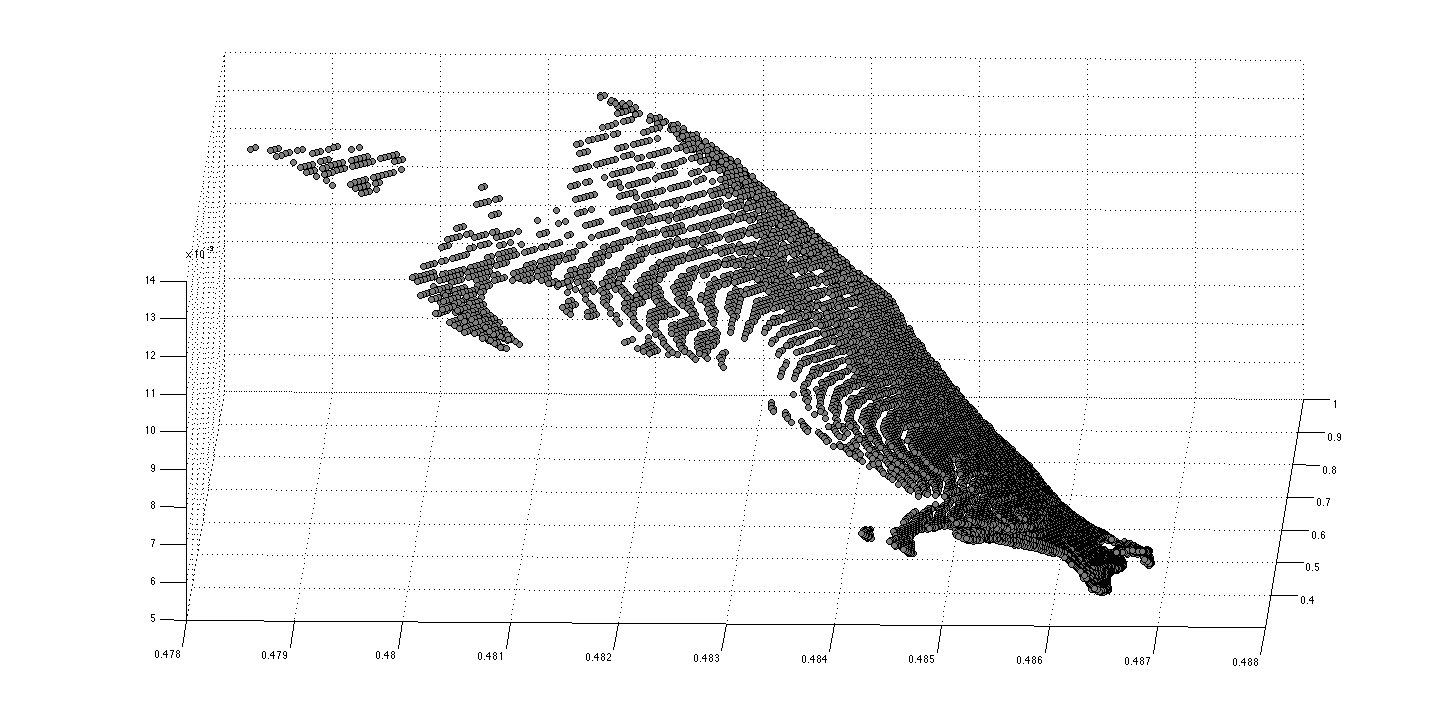
\includegraphics[width=\textwidth]{figures/rec_esti_1}
\caption{Visualization of the reconstructed 3d points (point-cloud) of the Cow model using our estimated translation and rotation transformation matrices. Viewing diagonally, from the size}
\label{fig:cow_rec_us_1}
\end{figure}

\begin{figure}[H]
\centering
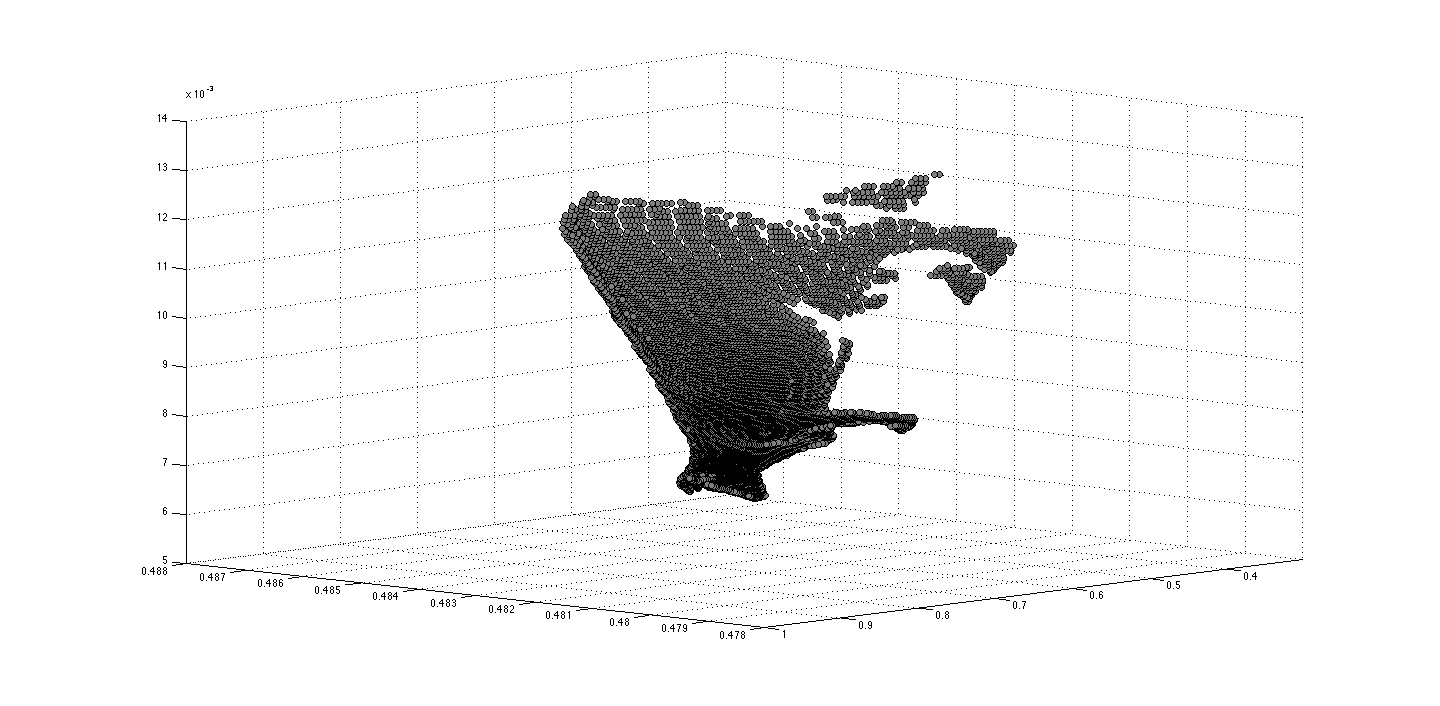
\includegraphics[width=\textwidth]{figures/rec_esti_2}
\caption{Visualization of the reconstructed 3d points (point-cloud) of the Cow model using our estimated translation and rotation transformation matrices. Viewing from the side, head downwards.}
\label{fig:cow_rec_us_2}
\end{figure}

\begin{figure}[H]
\centering
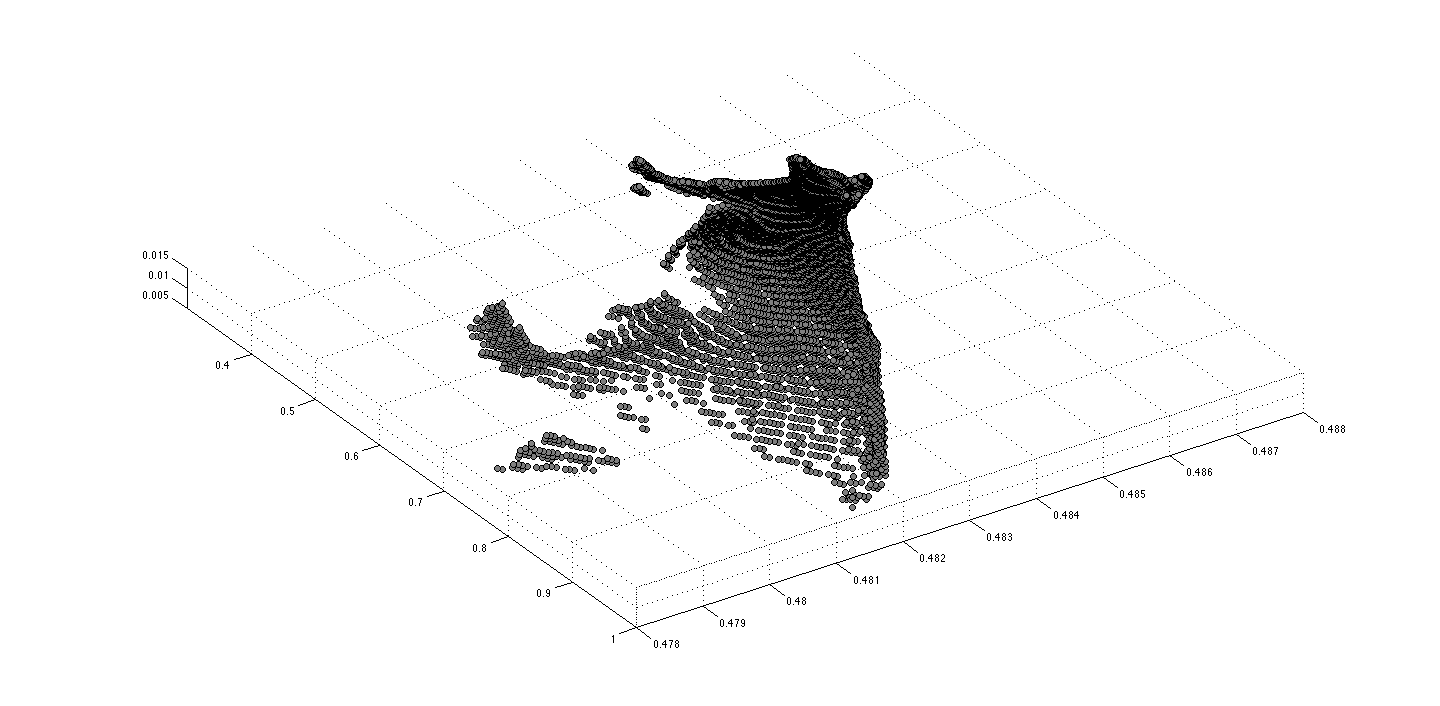
\includegraphics[width=\textwidth]{figures/rec_esti_3}
\caption{Visualization of the reconstructed 3d points (point-cloud) of the Cow model using our estimated translation and rotation transformation matrices. Viewing from top the side profile of the cow.}
\label{fig:cow_rec_us_3}
\end{figure}

\begin{figure}[H]
\centering
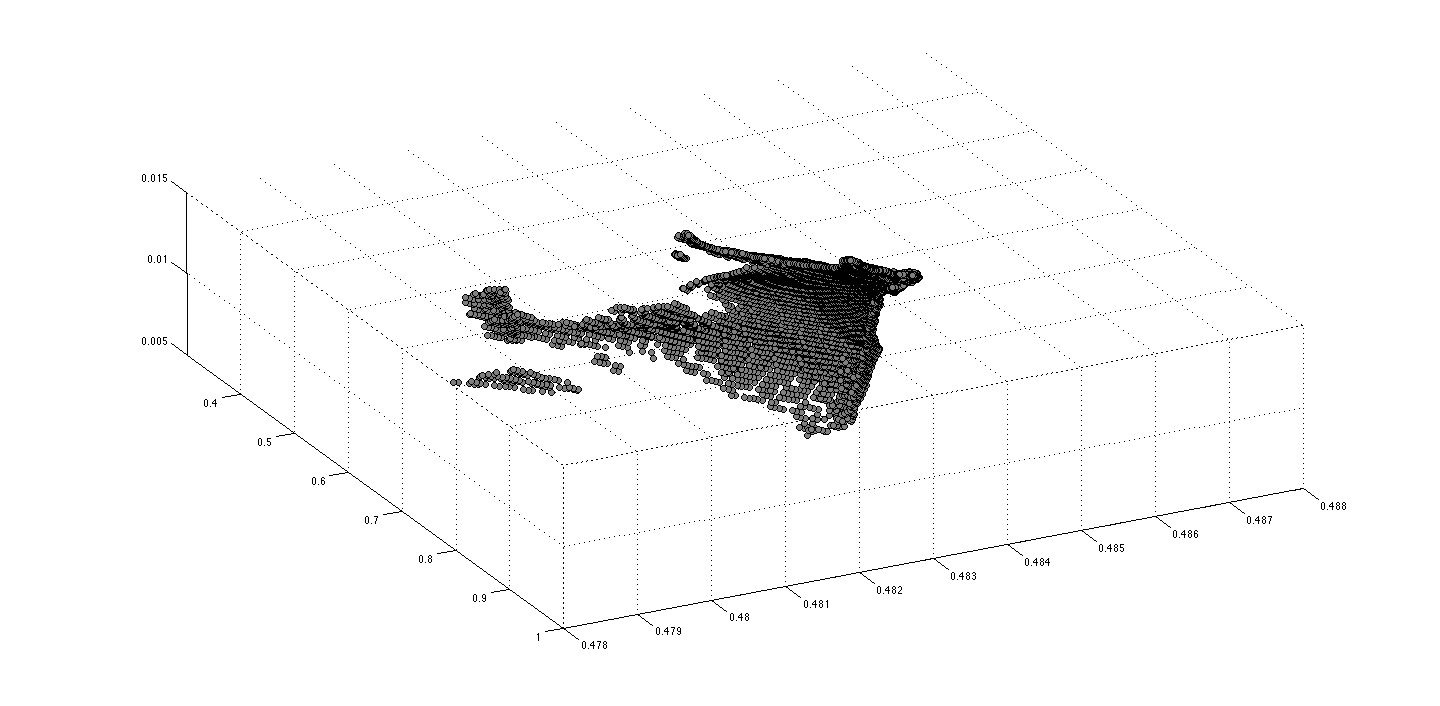
\includegraphics[width=\textwidth]{figures/rec_esti_4}
\caption{Visualization of the reconstructed 3d points (point-cloud) of the Cow model using our estimated translation and rotation transformation matrices. Viewing from top the side profile of the cow using a narrow angle in order to better recognize the width of the cow.}
\label{fig:cow_rec_us_4}
\end{figure}

% showing reconstruction using Rl and tl
\begin{figure}[H]
\centering
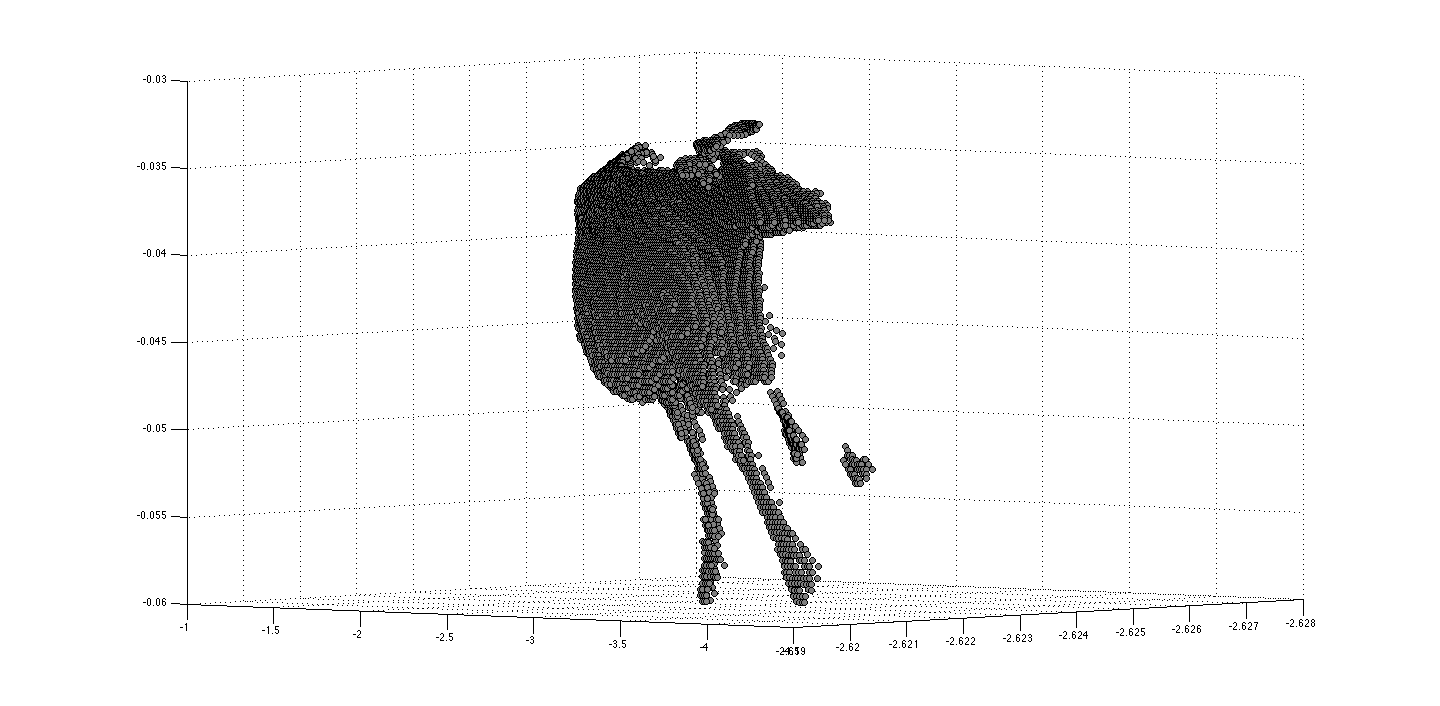
\includegraphics[width=\textwidth]{figures/rec_left_1}
\caption{Visualization of the reconstructed 3d points (point-cloud) of the Cow model using the provided $R_l$ and $t_l$}
\label{fig:cow_rec_rltl}
\end{figure}

% showing reconstruction using Rr and tr
\begin{figure}[H]
\centering
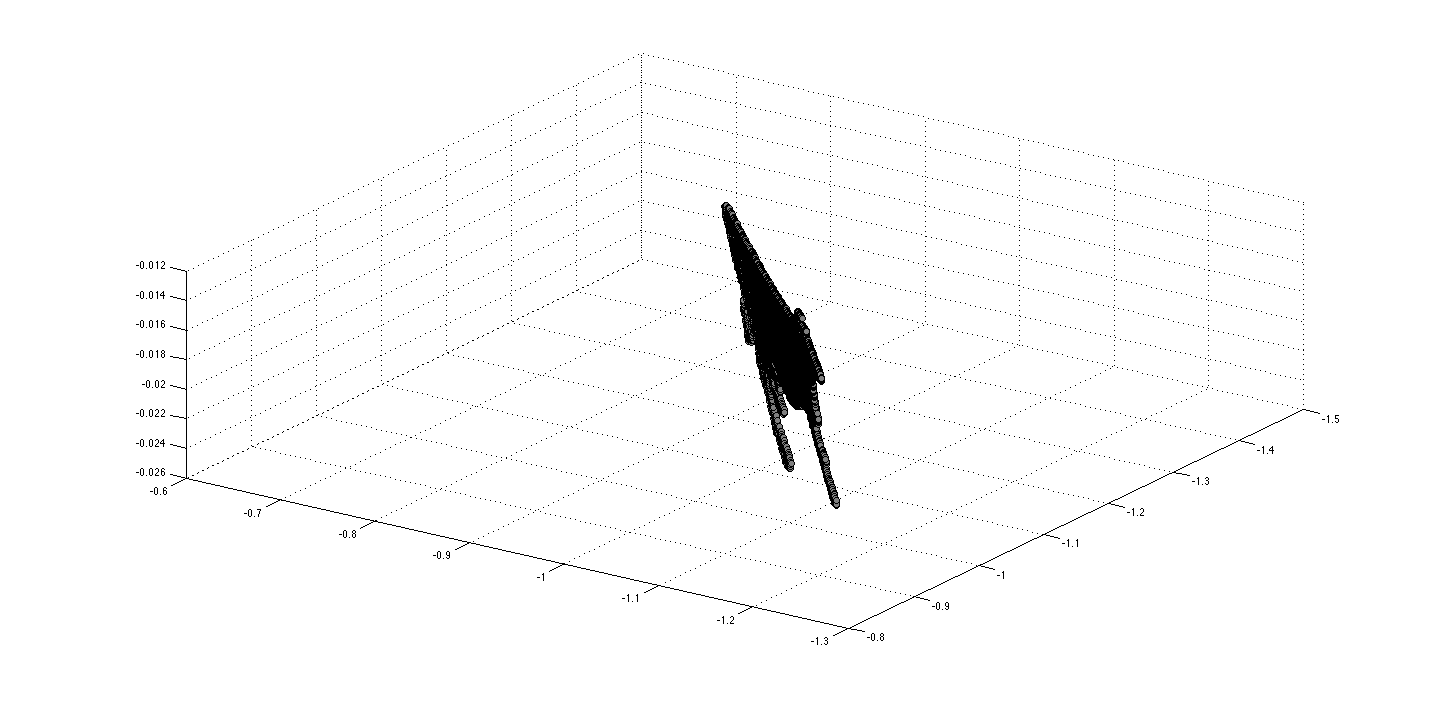
\includegraphics[width=\textwidth]{figures/rec_right_1}
\caption{Visualization of the reconstructed 3d points (point-cloud) of the Cow model using the provided $R_r$ and $t_r$}
\label{fig:cow_rec_rrtr}
\end{figure}



\end{document}